\section{Design and Implementation}
\label{sec:implementation}

This section discusses the implementation and design of \MP{}. It also discusses some common issues, such as adapting to different allocators, and the performance issue of collecting data. \MP{} profiles different aspects of memory allocators, such as performance overhead, memory overhead, scalability issue, and application friendliness. 

\MP{} is implemented as a library that should be preloaded before any other libraries, in order to intercept memory allocations/deallocations, memory-related system calls, and synchronizations. That also indicates that an allocator should utilize standard APIs in order to collect all relevant information. For instance, the Linux allocator utilizes the internal implementation of synchronizations by default.  For the profiling purpose, it should be changed to invoke explicit POSIX-APIs. Fortunately, most allocators do not need any change or the recompilation for the profiling.    

\subsection{Profiling Performance Overhead}

\label{sec:performanceimplement}

\MP{} profiles the performance overhead of every memory management operation. Since an allocator typically has different execution paths for different scenarios (as discussed in Section~\ref{sec:allocator}), such as new or re-used allocations, small or big objects, \MP{} further collects the information for each scenario separately. For allocation, \MP{} collects the data for new allocations of small objects, re-used allocations of small objects, and  allocations of big objects separately. For deallocation, \MP{} collects the deallocation data for small and big objects separately. 


The fine-grained data helps identify a particular design issue inside. For instance, DieHarder was found an serious performance issue for deallocating small objects, but with the normal performance for big objects, as further discussed in Section~\ref{}. Given the fine-grained data, programmers could only focus on the code relating to small objects. \MP{} relies on a configuration file to differentiate small from big objects, as further described in Section~\ref{sec:understandingallocators}, and differentiate re-used allocations from new allocations via a global hash map. All allocated addresses will be inserted into the global hash map.  If the address of an allocation can be found in the global hash map, then it is a re-used allocation. Otherwise, it is a new allocation.  

\MP{} collects the average time of each allocation and deallocation with the RDTSC instruction (Section~\ref{sec:pmu}), due to the performance and accuracy reason. Time stamps are taken before and after each operation, and then the difference between them is  the total number of cycles of an operation. 

\MP{} also employs the PMUs to collect hardware events of each operation, such as cache misses, page faults, TLB misses, and instructions. These hardware data are  significant supplements for identifying an issue, given that \MP{} is a non-intrusive profiler that cannot know the implementation details of an allocator. Let us revisit the issue of DieHarder. DieHarder is found to have a large number of cycles for its deallocation. But it is difficult to know the particular design issue inside, without more information. When given an unusual number of cache misses additionally, the issue related to the cache will be the main focus. Then programmers can easily identify the issue: DieHarder traverses all bags one by one to determine the original bag for an allocation, causing excessive number of cache misses. 

  
\subsection{Profiling Memory Overhead}
\label{sec:profilingmemory}

\MP{} collects real memory usage, real allocated memory, and total memory usage, when the memory usage of an application reaches its maximum value. However, it is very expensive to update these values for every new allocation. Therefore, \MP{} only updates the data when the total memory usage is increased by 1MB. For these data, real memory usage is the amount of memory actually requested by the application, where real allocated memory is the sum of real memory usage and internal fragmentation due to size-class based allocation. For example, if an application requests the memory by \texttt{malloc(454)}, then real memory usage is incremented by $454$, but real allocated memory will be incremented by the size of its corresponding class size. For this example, total memory will be incremented by page size instead (e.g., 4096 bytes), provided that the page was previously unused. 

\MP{} also collects different types of memory overhead, such as internal fragmentation, memory blowup, and others. It also collects the available memory and total memory consumption of each size class. The detailed data help programmers to pinpoint its memory overhead issue. For instance, if memory overhead mainly comes from the internal fragmentation, then the allocator should utilize more fine-grained size classes. If the memory overhead mainly comes from memory blowup, the allocator may require to adjust its synchronization frequency or take a more aggressive method for its synchronization~\citep{DBLP:conf/iwmm/LiLD19}. The memory overhead could be reduced with coalescence or splitting, if the major memory overhead comes from external fragmentation. 

\MP{} typically records different counters upon each allocation and deallocation. For the performance reason, \MP{} typically maintains a per-thread counter in order to reduce the contention issue. The per-thread counters includes the number of allocations and deallocations for each size class, the number of bytes for internal fragmentation, and allocated objects for each size class. 
\MP{} utilizes a global hash table to track the status information for each object, which is the same table for determining new or re-used object. Therefore, \MP{} could adjust the internal fragmentation upon each deallocation. 

\MP{} computes memory blowup for each size class at first, and then summarizes all of them as the total memory blowup. However, it is not intuitive to compute memory blowup. By definition, a new allocation will be treated as memory blowup, if there exist freed objects for this size class in other threads. However, the definition is not clear whether memory blowup should be reduced upon deallocations. \MP{} computes memory blowup for a size class based on the following observation: all freed objects of a size class is the \textit{upper bound} for its memory blowup; this upper bound deducted by recent freed objects will be the real memory blowup. In the implementation, \MP{} utilizes a global counter for each size class to track recent freed objects. This counter is incremented upon every deallocation, but will be decremented upon each allocation \textit{only} when the counter is larger than 0.  

 \MP{} reports other memory overhead as a summarized value, including external fragmentation, metadata overhead, and explicitly skipped objects. It is difficult to differentiate them without the implementation details. %Since \MP{} traps all memory usage requested by the allocator, the remaining memory except internal fragmentation and memory blowup will be reported. 
 

 
 %External fragmentation occurs when an allocator has sufficient memory but in a non-continuous way. Therefore, \MP{} keeps a global counter for the available memory, so that it could determine whether an allocation causes the external fragmentation issue or not.  The counter for the memory blowup will be incremented, if the current per-thread heap has no freed objects but there exit freed objects with the requested size class in other per-thread heaps. Therefore, \MP{} maintains a global counter for each size class. 

% Upon an allocation request, if the current thread does not possess any freed objects of the given size class -- but if the global counter does -- we record this event as an allocation responsible for increasing the allocator's memory blowup.

  
%  \todo{Based on the definitions of memory blowup and external fragmentation, an allocation will be counted as a memory blowup if there exists freed objects with the same size class. However, it is difficult to evaluate the external fragmentation. For instance, if freed objects with smaller class sizes exist, with the total size larger than the requested size, then the current allocation should be counted as external fragmentation. However, if freed objects with larger class sizes exist, it should not count as external fragmentation. But the overhead is caused by the issue of size class or without-splitting. Maybe we should make it clear in Section 3.3. }     
 

\subsection{Profiling Scalability}
\label{sec:profilingscale}

\MP{} also evaluates the scalability of a memory allocator. As described in Section~\ref{sec:scaleidea}, \MP{} evaluates the scalability for both user space and kernel space. 

For user-space scalability, \MP{} focuses on different types of locks, such as mutex locks, spin locks, and try locks. For each lock, \MP{} collects the number of acquisitions, the runtime of each acquisition (with the RDTSC instruction), the runtime of each critical section, the number of contentions, and the number of maximum contending threads. In order to obtain the information of contentions, \MP{} dynamically maintains the contention state of each lock. Upon the acquisition, \MP{} increments the contention threads of the corresponding lock, which will be decremented upon the release of this lock. In theory, the contention data is not accurate, since increments and decrements are not atomic. However,  the data could still show the contenting status of locks inside an allocator.    

For the kernel-space scalability, \MP{} focuses on memory-related system calls inside the allocation and deallocation, including \texttt{mmap}, \texttt{munmap}, \texttt{mremap}, \texttt{sbrk}, \texttt{madvise}, and \texttt{mprotect}. \MP{} profiles the runtime of each invocation with the RDSTC instruction, and the number of invocations for each system call. In fact, the simple data could actually uncover serious scalability issues of a memory allocator. For instance, the Linux allocator of \texttt{glibc-2.21} slows down an application by 40\%, which can be uncovered by the excessive number of \texttt{madvise} system calls and a higher runtime for the corresponding \texttt{mmap} and \texttt{mprotect} system call. In order to identify the data in specific execution path, \MP{} also collect the data for each type of allocations and deallocations, similar to the performance overhead of Section~\ref{sec:performanceimplement}.


\subsection{Application Friendliness}
\label{sec:profilefriendliness}

Currently, the Linux kernel has supported PMUs starting from 2009 (Linux-2.6.31)~\cite{pmulinuxsupport}, where users could set up performance monitoring via  the \texttt{perf\_event\_open} system call. After collecting events, the user program could fetch these events. 

\MP{} reports whether an allocator is friendly to a specific application. Different from all previous parts that only focusing inside memory management operations, application friendliness focuses on outside memory management operations. More specifically, \MP{} focuses on the following parameters, including (1)~the average cache line utilization; (2)~the average page utilization; (3)~the number of cache misses. As discussed in Section~\ref{sec:friendliness}, a user-friendly allocator should have high cache-line and page utilization rates, but with a low number of cache misses.  

\MP{} employs the PMU-based sampling to track the average cache utilize and page utilization. Basically, \MP{} samples memory accesses periodically, with a default sampling period of 5,000. Upon every sampled event, \MP{} collects the number of used bytes for the current cache line and the current page, and also increments the number of sampled cache lines and pages. In the end, \MP{} computes the utilization rate with a simple division. For cache utilization rate, the dividend is the total number of used bytes, and the divisor is the the total number of bytes for these cache lines. The page utilization rate is computed similarly, but focusing on the page level instead. 

However, the challenge is to quickly locate the  metadata for each cache line and each page, since the metadata should be updated upon every allocation and deallocation, and upon every sampled event. During its implementation, \MP{} has tried multiple mechanisms. First, \MP{} designed a red-black tree to hold memory mappings of the heap, and then stored the address of corresponding metadata on the tree node. This mechanism was found to be in-efficient, since some allocators (e.g., OpenBSD) includes thousands of mappings, which may introduce tens of comparisons unfortunately. Second, \MP{} utilized a hash map to store the memory mappings. But it is difficult to decide the right number of buckets for the hash table, where a small number may cause too many conflicts, with significant performance overhead by traversing the link list.  Finally, \MP{} designs a fast lookup mechanism by taking advantage of the vast address space of 64-bits machines, where the detailed design is discussed as follows. 

% Based on our observation, all allocators invoke either \texttt{sbrk} or \texttt{mmap} system calls to obtain the memory from the underlying OS. The address range returned from \texttt{sbrk} is generally lower than 4G, while the range returned by \texttt{mmap} is typically less than 128TB. 
%Given that modern processors typically support 48 bits address space (256 TB), \MP{} employs the last TB (between 255TB and 256TB) of address space to store the meta data of object, with the design illustrated in Figure~\ref{fig:lookup}. 

\textbf{Three-Level Fast Lookup Mechanism:} \MP{} designs a three-level lookup mechanism as illustrated in Fig.~\ref{fig:lookup}, borrowing the idea of multi-level page table design of OS. Basically, a ``MB Mapping'' will be the first level, where the index can be computed simply by dividing an address with 1 megabytes (MB). Each entry of this MB mapping points to all possible pages inside the current 1-megabyte memory. Since one MB memory will have at most 256 pages, with the size of 4KB for each page, each MB entry points to 256 page entries. Similarly, each page entry has the information about used bytes in this page and has a pointer pointing to 64 possible cache entries inside. Based on this design, it takes two steps to get the used bytes for a page, and takes three steps to get the used bytes for the current cache line. Therefore, it has the $\mathcal{O}(1)$ 
complexity to obtain the metadata.  
          
\begin{figure*}[!h]
\centering
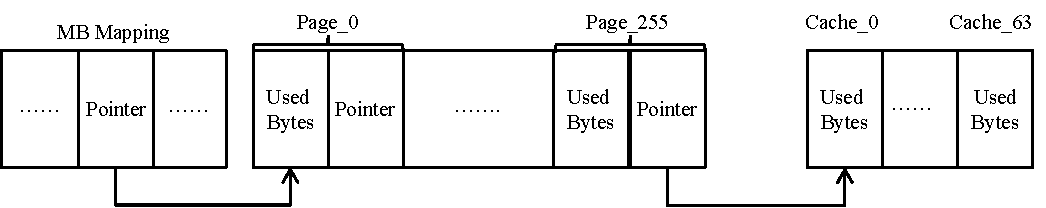
\includegraphics[width=5.5in]{figures/lookup}
\caption{Three-level Lookup Mechanism.\label{fig:lookup}}
\end{figure*}

Note that this design is also efficient in memory consumption. If a range of addresses are not used, then there is no need to allocate physical memory for the corresponding page entries and cache entries. This design is able to adapt to different allocators, where memory mappings of a heap is varied from a few to hundreds of thousands, and these mappings can be scattered along the whole address space of a process. To track valid memory mappings dynamically, \MP{} intercepts memory related system calls inside allocations/deallocations, such as \texttt{sbrk}, \texttt{mmap}, \texttt{munmap}, \texttt{mremap}. 

\subsection{Predicting Performance Impact}
\label{sec:predict}

\subsection{Adapting To Different Allocators}
\label{sec:understandingallocators}

\MP{} is designed as a general profiler for sequential and BiBOP-style allocators, as described in Section~\ref{sec:allocator}. The challenge is to adapt  to different allocators. \MP{} interprets a configuration file to identify the difference of every allocator in its initialization phase, such as the allocator's style (BiBOP-style versus sequential), sizes of different classes, the threshold of separating small objects from large objects. This configuration can be provided manually. \MP{} also provides a prerun program to understand these details of an allocator. 

In order to identify the style of allocator, the prerun routine will check whether two subsequent allocations with different sizes (small objects, apparently from different size classes) are allocated from the same page or not. If yes, then the allocator is a sequential-style allocator, which is similar to the default Linux allocator. Otherwise, the allocator belongs to a BiBOP-style allocator. 

The second step is to identify the sizes of different size classes. The prerun routine begins by allocating an object of 8 bytes, and continues to allocate additional objects using a stride increase of 8 bytes each time. The determination of size classes depends on the style of an allocator. For BiBOP-style allocators, an allocation with a different size class will be satisfied from a different bag, locating in a different page. For sequential allocators, such as the Linux allocator, the distance between two contiguously-allocated objects (with distinct sizes) is utilized to determine the size class. As shown in Fig.~\ref{fig:sizeclass}, if the size of $Obj_1$ and $Obj_2$ is the same, judging from the distance of between two continuous objects, then they belong to the same size class. Otherwise, they belong to different size class, such as $Obj_3$ in the figure. By checking the size of two objects belonging to different objects, we could determine the sizes of different size classes.  

\begin{figure}[!ht]
\centering
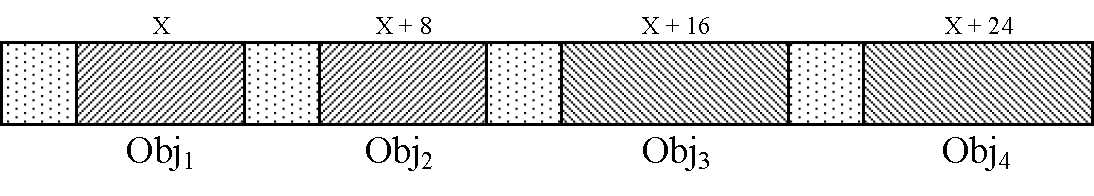
\includegraphics[width=5in]{figures/sequentialclasssize}
\caption{Determining the size class of a sequential allocator by the distance between continuous allocations. \\The boxes with 10\% dotted pattern are the metadata, and the boxes with diagonal stripes\\ are actual heap objects. The number above every box is the size of the corresponding object. \label{fig:sizeclass}}
\end{figure}


The threshold for big objects are typically detected by checking whether there is an explicit \texttt{mmap} system calls upon the allocation. Typically, most allocators utilize a direct \texttt{mmap} system call to satisfy the allocation for a big object initially. However, this threshold requires the manual confirmation. 

